
\chapter{Arhitektura i dizajn sustava}
		
		
	\noindent Komunikacija sa našim sustavom ostvaruje se korištenjem web preglednika koji prikazuje grafičko sučelje naše aplikacije. Korisnička interakcija sa grafičkim sučeljem rezultira slanjem zahtjeva web preglednika prema web poslužitelju na kojem se nalazi naša web aplikacija. \newline
	Iz navedenog možemo definirati \textbf{web preglednik} kao program koji krajnjem korisniku omogućava jednostavno pretraživanje i pregled podataka na Internetu, \textbf{web poslužitelj} kao program koji prima zahtjeve web preglednika, prosljeđuje ih web aplikaciji na obradu te odgovara web pregledniku podacima koji su mu proslijeđeni od strane web aplikacije. \textbf{Web aplikacija} program je koji obrađuje primljene zahtjeve, komunicira s bazom podataka te šalje podatke web poslužitelju za prikaz u web pregledniku.
	\newline 
	U našem slučaju web poslužitelju se pristupa putem REST-a (engl. \textit{Representational State Transfer}) te je odgovor poslužitelja u JSON obliku.
	\newline
	Troslojna arhitektura našeg sustava prezentirana je sljedećim slojevima
	\begin{packed_item}
		\item Sloj interakcije
		\item Sloj servisa
		\item Sloj repozitorija
	\end{packed_item}
	
	
	\noindent Interakcijski sloj predstavlja sučelje aplikacije pomoću kojeg krajnji korisnik iskorištava ostvarene funkcionalnosti aplikacije. 
	\newline 
	Sastoji se od dva podsloja:
	\begin{packed_item}
		\item Prikazni sloj
		\item Kontrolerski sloj 
	\end{packed_item}
	
	\noindent Prikazni sloj dio je \textit{frontend} dijela sustava. Za njegovu implementaciju odabran je React razvojni okvir (engl. \textit{framework}). \newline
	Kontrolerski sloj dio je \textit{backend} dijela sustava. Zadužen je za posluživanje zahtjeva dobivenih od prikaznog sloja.
	\newline\newline
	Servisni sloj naše aplikacije sadržan je unutar \textit{backend} dijela sustava. Sadrži strukture i funkcije čija je zadaća ispunjavanje zamišljenih funkcionalnosti aplikacije. Unutar njega se odrađuju izračuni i obrada podataka koji se onda predaju podatkovnom sloju. \newline\newline
	Repozitorijski je sloj također sadržan unutar već navedenog \textit{backend} dijela sustava. Zadužen je za komunikaciju s bazom podataka i razmjenom navedenih podataka sa servisnim slojem.
	\newline\newline
	Navedeni opis slojeva odgovara MVC arhitekturi (engl. \textit{Model-View-Controller}) čija je osnovna forma prikazana na sljedećoj slici. \newline
	\begin{figure}[H]
		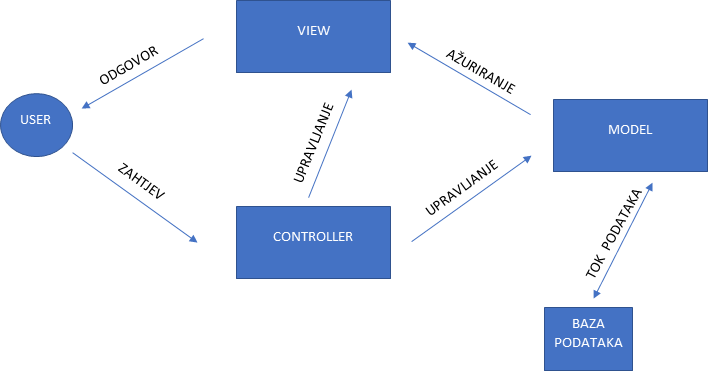
\includegraphics[scale=0.6]{./Slike/mvc-opce.png}
		\centering
		\caption{Opći MVC obrazac}
		\label{fig:promjene}
	\end{figure}
	\noindent Korištenjem Spring razvojnog okvira (engl. \textit{framework}) za razvoj aplikacije sloj prikaza i sloj kontrolera spojeni su unutar jednog sloja (koji možemo zvati sloj interakcije), dok su ostala dva sloja ostala odvojena. 
	\begin{figure}[H]
		
\includegraphics[scale=0.6]{./Slike/mvc-spring.png}
		\centering
		\caption{Spring MVC obrazac}
		\label{fig:promjene}
	\end{figure}
	\noindent Svi navedeni slojevi ostvaruju svoje funkcionalnosti komunikacijom s modelima (engl. models) sustava. Oni su oblikovani na način da apstrahiraju korisnike i elemente sustava te enkapsuliraju atribute potrebne za ostvarenje zamišljenih funkcionalnosti sustava. 
	\newline 
	Spring razvojni okvir (engl. \textit{framework}) pohranjuje strukturu modela unutar baze podataka korištenjem objektno-relacijskog preslikavanja (engl. \textit{object-relational mapping, ORM}) koje pruža alat Hibernate ORM. Preslikavanje se odvija prema predodređenim Java specifikacijama unutar Java Persistence aplikacijskog sučelja (JPA) koje alat kao što je Hibernate ORM implementira. Rezultat je skup tablica unutar odabrane baze podataka koje sadrže atribute modela i atribute veza među modelima.
	\newline
	Sustav upravljanja bazama podataka (engl. \textit{Relation Database Management System, RDBMS}) koji smo odabraili za izradu aplikacije je PostgreSQL. Jednostavno ga je integrirati unutar Spring razvojnog okvira (engl. \textit{framework}) uključivanjem tzv. \textit{dependecya}.
	
			
	\section{Baza podataka}
		
		
	Za potrebe sustava modelirana je relacijska baza podataka koja svojom strukturom modelira stvarni svijet, tj. odnose potrebne aplikaciji. Gradivna jedinka baze je relacija,  tablica definirana svojim imenom i skupom atributa. Zadaća baze podataka brza je i jednostavna pohrana, izmjena i dohvat podataka za daljnju obradu.
	Baza podataka ove aplikacije sastoji se od sljedećih entiteta:
	\begin{packed_item}
		\item User
		\item Client
		\item Coach
		\item Training
		\item Workout
		\item Time
		\item Goals
		\item Schedule
		\item Token
		\item Training\_workouts
		\item Client\_schedules
		\item Coach\_clients
		\item Client\_trainings
	
	\end{packed_item}
	
		\subsection{Opis tablica}
	
	
			\textbf{USER} \newline
	Entitet USER sadržava informacije o korisniku aplikacije. Korisnik može biti trener, klijent i administrator. Sadrži atribute: userID, name, surname, dateOfBirth, username, email, password, contact, role. 
			
			\begin{longtblr}[
				label=none,
				entry=none
				]{
					width = \textwidth,
					colspec={|X[6,l]|X[6, l]|X[20, l]|}, 
					rowhead = 1,
				} %definicija širine tablice, širine stupaca, poravnanje i broja redaka naslova tablice
				\hline \multicolumn{3}{|c|}{\textbf{USER}}	 \\ \hline[3pt]
				\SetCell{LightGreen} userID & BIGINT	&  	jedinstveni identifikator korisnika  	\\ \hline
				name & VARCHAR & ime korisnika		\\ \hline 
				surname & VARCHAR & prezime korisnika	\\ \hline 
				dateOfBirth & DATE & datum rođenja korisnika \\ \hline
				email & VARCHAR & e-mail adresa korisnika \\ \hline 
				username & VARCHAR & korisničko ime korisnika, alternativni ključ  	\\ \hline 
				password & VARCHAR & hash zapis lozinke	\\ \hline 
				contact & VARCHAR & kontakt broj korisnika \\ \hline
				role & ENUM	& uloga korisnika u sustavu	\\ \hline 
			\end{longtblr}
			
			\textbf{CLIENT} \newline
	Entitet CLIENT predstavlja specijalizaciju nad entitetom USER. Sadrži atribute entitete USER te currentGoal, nextGoal, hoursAvailable.
			
			\begin{longtblr}[
				label=none,
				entry=none
				]{
					width = \textwidth,
					colspec={|X[6,l]|X[6, l]|X[20, l]|}, 
					rowhead = 1,
				} %definicija širine tablice, širine stupaca, poravnanje i broja redaka naslova tablice
				\hline \multicolumn{3}{|c|}{\textbf{CLIENT}}	 \\ \hline[3pt]
				\SetCell{LightBlue} currentGoal & VARCHAR & trenutni cilj \\ \hline
				\SetCell{LightBlue} nextGoal & VARCHAR & sljedeći odabrani cilj \\ \hline
			 hoursAvailable & INT & fond sati treninga po mjesecu \\ \hline
			\end{longtblr}
			
			\textbf{COACH} \newline
	Entitet COACH predstavlja specijalizaciju nad entitetom USER. Sadrži atribute eniteta USER i atribut verified koji predstavlja odobrenje administratora
			
			\begin{longtblr}[
				label=none,
				entry=none
				]{
					width = \textwidth,
					colspec={|X[6,l]|X[6, l]|X[20, l]|}, 
					rowhead = 1,
				} %definicija širine tablice, širine stupaca, poravnanje i broja redaka naslova tablice
				\hline \multicolumn{3}{|c|}{\textbf{COACH}}	 \\ \hline[]
				\hline verified & BOOLEAN	&  status verifikacije trenera  	\\ \hline
				
			\end{longtblr}
		
			\textbf{TRAINING} \newline
	Entitet TRAINING sadržava informacije o treningu. Sadrži atribute: trainingID, userID, trainingName, duration, trainingRules. Entitet je u vezi Many-to-Many s entitetom TRAINING\_WORKOUTS preko atributa trainingID.
			
			\begin{longtblr}[
				label=none,
				entry=none
				]{
					width = \textwidth,
					colspec={|X[6,l]|X[6, l]|X[20, l]|}, 
					rowhead = 1,
				} %definicija širine tablice, širine stupaca, poravnanje i broja redaka naslova tablice
				\hline \multicolumn{3}{c}{\textbf{TRAINING}}	 \\ \hline[3pt]
				\SetCell{LightGreen} trainingID & INT	&  	jedinstveni identifikator treninga  	\\ \hline
				\SetCell{LightBlue}coachUserID & INT & jedinstveni identifikator trenera \\ \hline 
				trainingName & VARCHAR & naziv treninga 	\\ \hline 
				duration & TIME & duljina treninga \\ \hline 
				trainingRules & VARCHAR & pravila koja postavlja trener\\ \hline 
			\end{longtblr}
		
			\textbf{WORKOUT} \newline
	Entitet WORKOUT sadržava sve moguće vježbe unutar aplikacije. Sadrži atribute: workoutID, workoutName, workoutTypeID. Entitet je u vezi Many-To-Many s TRAINING\_WORKOUTS preko atributa workoutID, te u vezi Many-To-One s WORKOUT\_TYPE preko atributa workoutTypeID;
		
			\begin{longtblr}[
				label=none,
				entry=none
				]{
					width = \textwidth,
					colspec={|X[6,l]|X[6, l]|X[20, l]|}, 
					rowhead = 1,
				} %definicija širine tablice, širine stupaca, poravnanje i broja redaka naslova tablice
				\hline \multicolumn{3}{|c|}{\textbf{WORKOUT}}	 \\ \hline[3pt]
				\SetCell{LightGreen} workoutID & INT	&  	jedinstveni identifikator vježbe  	\\ \hline
				workoutName & VARCHAR & naziv vježbe 	\\ \hline 
				workoutTypeID & BIGINT & identifikator tipa vježbe \\ \hline 
			\end{longtblr}
		
			\textbf{TIME} \newline
	Entitet TIME sadržava moguće termina treninga unutar dana. Sadrži atribut timeOfday. 
			
			\begin{longtblr}[
				label=none,
				entry=none
				]{
					width = \textwidth,
					colspec={|X[6,l]|X[6, l]|X[20, l]|}, 
					rowhead = 1,
				} %definicija širine tablice, širine stupaca, poravnanje i broja redaka naslova tablice
				\hline \multicolumn{3}{|c|}{\textbf{TIME}}	 \\ \hline[3pt]
				\SetCell{LightGreen} timeOfDay & INT & termin treninga unutar dana  	\\ \hline
			\end{longtblr}	
		
			\textbf{GOALS} \newline
	Entitet GOALS sadržava moguće ciljeve vježbanja za korisnika. Sadrži atribute goalName.
			
			\begin{longtblr}[
				label=none,
				entry=none
				]{
					width = \textwidth,
					colspec={|X[6,l]|X[6, l]|X[20, l]|}, 
					rowhead = 1,
				} %definicija širine tablice, širine stupaca, poravnanje i broja redaka naslova tablice
				\hline 
				\multicolumn{3}{c}{\textbf{GOALS}}	 \\ \hline[3pt]
				\SetCell{LightGreen} goalName & VARCHAR & jedinstveni identifikator i naziv cilja  	\\ \hline
			\end{longtblr}	
			
			\textbf{SCHEDULE} \newline
	Entitet SCHEDULE sadržava informacije o održavanju treninga unutar dana, te broju mjesta slobodnih za određeni trening. Sadrži atribute trainingID, date, timeOfDay, spaceLeft. TrainingID strani je ključ entiteta TRAINING te s atributom date čini primarni ključ.
			
			\begin{longtblr}[
				label=none,
				entry=none
				]{
					width = \textwidth,
					colspec={|X[6,l]|X[6, l]|X[20, l]|}, 
					rowhead = 1,
				} %definicija širine tablice, širine stupaca, poravnanje i broja redaka naslova tablice
				\hline 
				\multicolumn{3}{c}{\textbf{SCHEDULE}}	 \\ \hline[3pt]
				\SetCell{LightGreen} trainingID & BIGINT & jedinstveni identifikator treninga 	\\ \hline
			  \SetCell{LightGreen} date & DATE & datum treninga \\ \hline
			  \ timeOfDay & INT & termin treninga u danu \\ \hline
			  \ spaceLeft & INT & broj slobodnih mjesta \\ \hline
			  \end{longtblr}
			  
	% 		   \textbf{TOKEN} \newline
	% Entitet TOKEN sadržava informacije o novoregistriranom korisniku i generiranom tokenu (string) koji mu je dodijeljen za mail verifikaciju.
		  
	% 		\begin{longtblr}[
	% 			label=none,
	% 			entry=none
	% 			]{
	% 				width = \textwidth,
	% 				colspec={|X[15,l]|X[6, l]|X[20, l]|}, 
	% 				rowhead = 1,
	% 			} %definicija širine tablice, širine stupaca, poravnanje i broja redaka naslova tablice
	% 			\hline 
	% 			\multicolumn{3}{c}{\textbf{TOKEN}}	 \\ \hline[3pt]
	% 			\SetCell{LightGreen} tokenID & BIGINT & jedinstveni identifikator tokena	\\ \hline
	% 		  \SetCell{LightBlue} userID & BIGINT & jedinstveni identifikator korisnika \\ \hline
	% 		  \ token & VARCHAR & token \\ \hline
	% 		  \end{longtblr} 
			  
	\textbf{TRAINING\_WORKOUTS} \newline
	TRAINING\_WORKOUTS predstavlja spojnu tablicu treninga i vježbi koja će se koristiti za određivanje vrste treninga. Sadrži atribute trainingID i workoutID koji su strani ključevi redom tablica TRAINING i WORKOUT.
		  
			\begin{longtblr}[
				label=none,
				entry=none
				]{
					width = \textwidth,
					colspec={|X[15,l]|X[6, l]|X[20, l]|}, 
					rowhead = 1,
				} %definicija širine tablice, širine stupaca, poravnanje i broja redaka naslova tablice
				\hline 
				\multicolumn{3}{c}{\textbf{TRAINING\_WORKOUTS}}	 \\ \hline[3pt]
				\SetCell{LightGreen} trainingID & BIGINT & jedinstveni identifikator treninga 	\\ \hline
			  \SetCell{LightGreen} workoutID & BIGINT & jedinstveni identifikator vježbe \\ \hline
			  \end{longtblr}
			  
			\textbf{CLIENT\_SCHEDULES} \newline
	CLIENT\_SCHEDULES predstavlja spojnu tablicu koja povezuje klijenta s dodijeljenim treninzima i njihovim terminima. Sadrži atribute userID, trainingID, date, reservation. UserID i trainingID redom su strani ključevi iz tablica USER i TRAINING.
		  
			\begin{longtblr}[
				label=none,
				entry=none
				]{
					width = \textwidth,
					colspec={|X[15,l]|X[6, l]|X[20, l]|}, 
					rowhead = 1,
				} %definicija širine tablice, širine stupaca, poravnanje i broja redaka naslova tablice
				\hline 
				\multicolumn{3}{c}{\textbf{CLIENT\_SCHEDULES}}	 \\ \hline[3pt]
				\SetCell{LightGreen} userID & BIGINT & jedinstveni identifikator korisnika 	\\ \hline
			  \SetCell{LightGreen} trainingID & BIGINT & jedinstveni identifikator treninga \\ \hline
			  \SetCell{LightGreen} date & DATE & datum treninga \\ \hline
			  \ reservation & BOOLEAN & potvrda rezervacije termina treninga \\ 
			  \hline
			  \end{longtblr}
		  
			\textbf{COACH\_CLIENTS} \newline
	COACH\_CLIENTS predstavlja spojnu tablicu koja povezuje trenera sa svojim klijentima. Sadrži atribute coachID, clientID. CoachID i ClientID redom su strani ključevi iz tablica COACH i CLIENT u kojima se pojavljuju kao userID.
		  
			 \begin{longtblr}[
				label=none,
				entry=none
				]{
					width = \textwidth,
					colspec={|X[15,l]|X[6, l]|X[20, l]|}, 
					rowhead = 1,
				} %definicija širine tablice, širine stupaca, poravnanje i broja redaka naslova tablice
				\hline 
				\multicolumn{3}{c}{\textbf{COACH\_CLIENTS}}	 \\ \hline[3pt]
				\SetCell{LightGreen} coachID & BIGINT & jedinstveni identifikator trenera 	\\ \hline
			  \SetCell{LightGreen} clientID & BIGINT & jedinstveni identifikator klijenta \\ \hline
			  \end{longtblr}                
			  
			\textbf{CLIENT\_TRAININGS} \newline
	CLIENT\_TRAININGS predstavlja spojnu tablicu koja povezuje klijenta sa dodijeljenim treninzima. Sadrži atribute userID te trainingID. UserID i trainingID redom su strani ključevi iz tablica CLIENT i TRAINING.
		  
			 \begin{longtblr}[
				label=none,
				entry=none
				]{
					width = \textwidth,
					colspec={|X[15,l]|X[6, l]|X[20, l]|}, 
					rowhead = 1,
				} %definicija širine tablice, širine stupaca, poravnanje i broja redaka naslova tablice
				\hline 
				\multicolumn{3}{c}{\textbf{CLIENT\_TRAININGS}}	 \\ \hline[3pt]
				\SetCell{LightGreen} userID & BIGINT & jedinstveni identifikator klijenta  	\\ \hline
			  \SetCell{LightGreen} trainingID & BIGINT & jedinstveni identifikator treninga \\ \hline
			  \end{longtblr}    
			  \textbf{WORKOUT\_TYPE} \newline
	WORKOUT\_TYPE predstavlja tablicu koja sadrži podatke o mogućim tipovima vježbi. Sadrži atribute typeID i workoutType.
		  
			 \begin{longtblr}[
				label=none,
				entry=none
				]{
					width = \textwidth,
					colspec={|X[15,l]|X[6, l]|X[20, l]|}, 
					rowhead = 1,
				} %definicija širine tablice, širine stupaca, poravnanje i broja redaka naslova tablice
				\hline 
				\multicolumn{3}{c}{\textbf{WORKOUT\_TYPE}}	 \\ \hline[3pt]
				\SetCell{LightGreen} typeID & BIGINT & jedinstveni identifikator tipa vježbe  	\\ \hline
			  \ workoutType & VARCHAR & naziv tipa vježbe \\ \hline
			  \end{longtblr}               
		  
		  
		  
		  
		  
		\subsection{Dijagram baze podataka}
			\begin{figure}[H]
		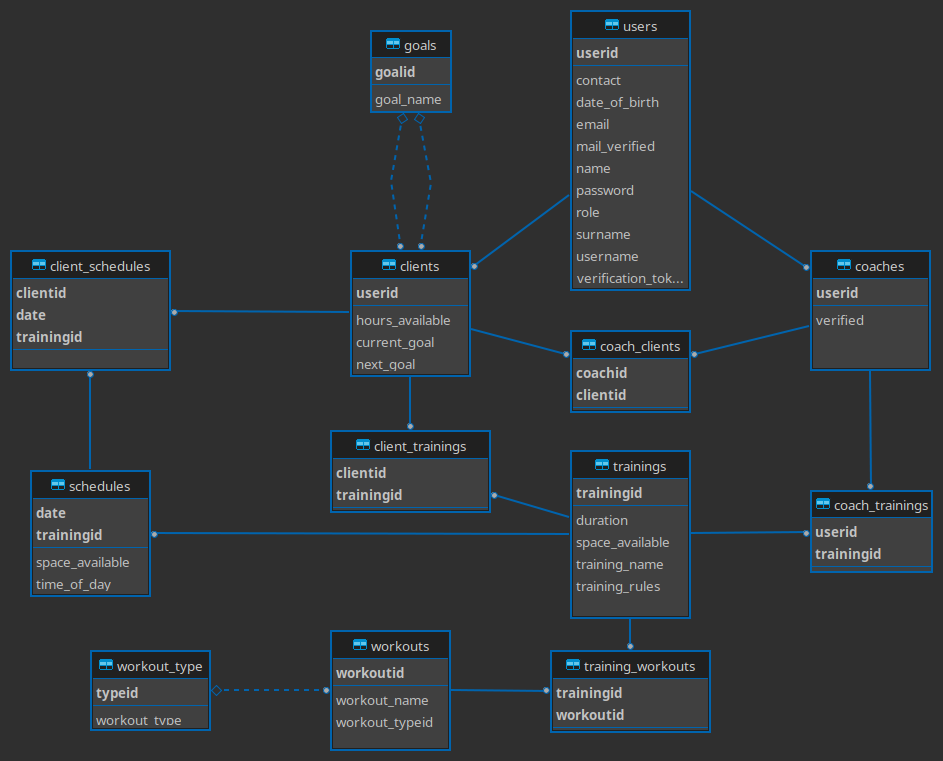
\includegraphics[scale=0.45]{./Dijagrami/relations.png}
		\centering
		\caption{Dijagram tablica unutar baze podataka}
		\label{fig:promjene}
	\end{figure}
		
		\eject
		
		
	\section{Dijagram razreda}
		\noindent Dijagrami razreda pokazuju povezanost komponenti sustava te daju jasniji uvid u arhitekturu i dizajn aplikacije. Podijeljeni su u 4 podkategorije (sa dodatnim prikazom metoda servisa) :
		 \begin{packed_item}    
			\item Modeli - Slika 4.4
			\item Kontroleri u vezi sa servisima - Slika 4.5
			\item Servisi u vezi sa repozitorijima - Slika 4.6                
			\item Repozitoriji - Slika 4.7
                \item Servisi - Slika 4.8
		
		\end{packed_item}
		\noindent U modelima je važno istaknuti postojanje glavne klase za korisnike zvane "User". Iz nje su izvedene klase klijenta (vježbač) i trenera sa potrebnim atributima specijalizacije.
		\begin{figure}[H]
		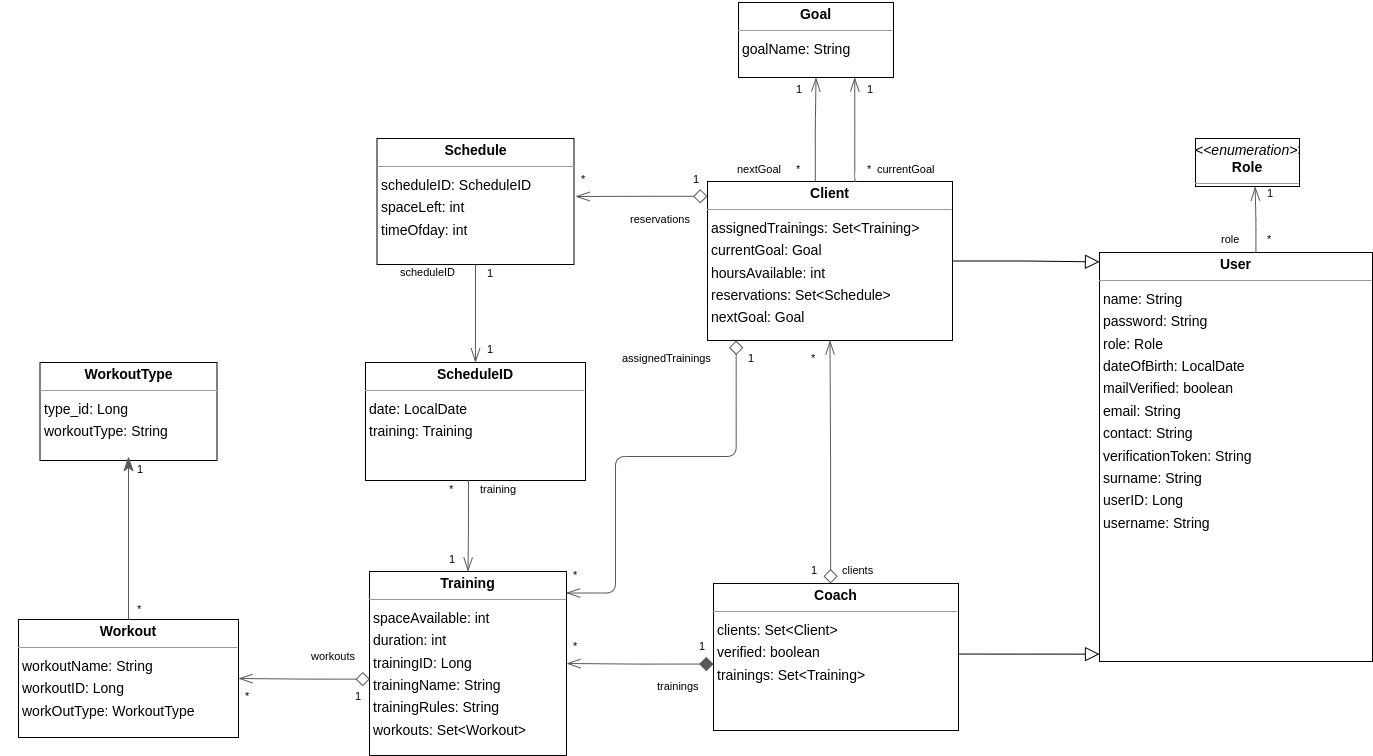
\includegraphics[scale=0.425]{./Dijagrami/domain.png}
		\centering
		\caption{Modeli}
		\label{fig:promjene}
	\end{figure}
    \noindent Servisi ostvaruju funkcionalnosti sustava komunikacijom sa bazom podataka preko repozitorija. Prikazani su neki glavni servisi (i njihove implementacije) koji su zaduženi za opće korisnike (tj. funkcionalnosti koje imaju i klijenti i treneri) te pojedinačni servisi za svaku od navedenih uloga.
	\begin{figure}[H]
		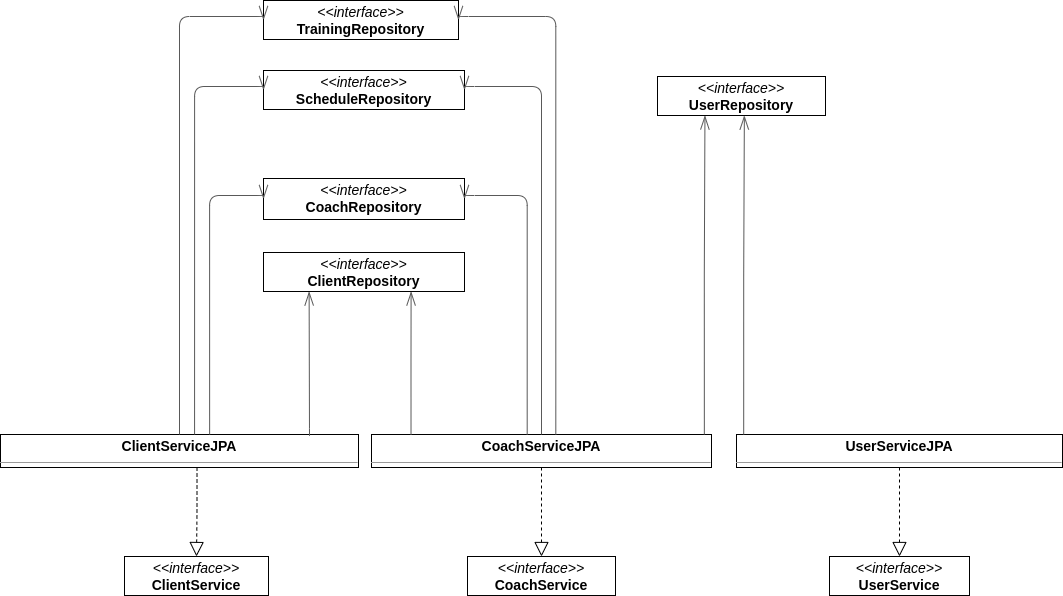
\includegraphics[scale=0.425]{./Dijagrami/services_repositories.png}
		\centering
		\caption{Servisi u vezi sa repozitorijima}
		\label{fig:promjene}
	\end{figure}
	\noindent Kontroleri i servisi čine najvažniji dio sustava jer sadržavaju logiku potrebnu za ostvarivanje zamišljenih funkcionalnosti. Dobivanjem zahtjeva sa \textit{frontend} strane sustava, kontroleri prosljeđuju iste odgovarajućim servisima (sa kojima su u vezi). Ovdje su prikazani najvažniji servisi (i odgovarajuće implementacije) i kontroleri za ostvarivanje funkcionalnosti trenera, klijenata i korisnika kao zajedničkog naziva istih.
	\begin{figure}[H]
		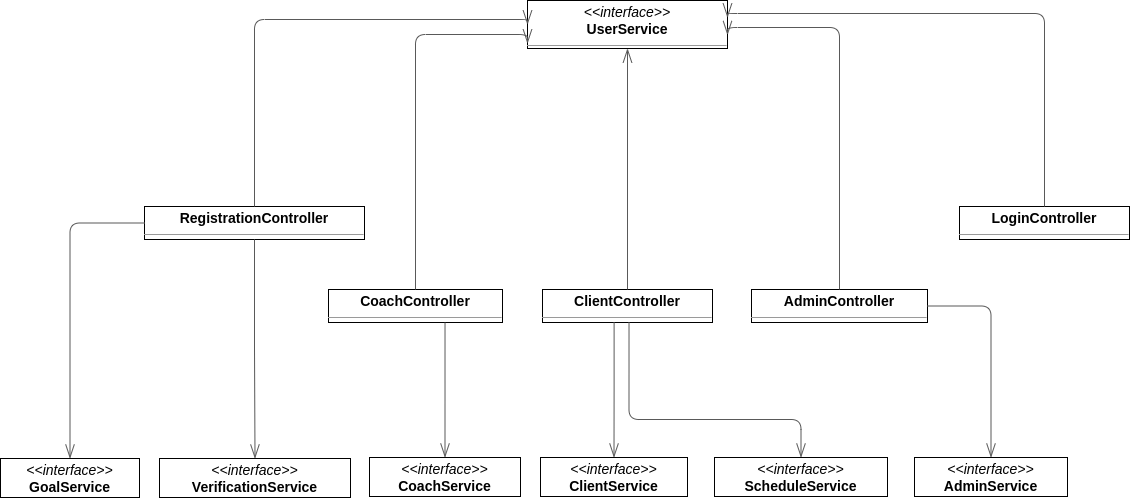
\includegraphics[scale=0.4]{./Dijagrami/controllers_services.png}
		\centering
		\caption{Kontroleri u vezi sa servisima}
		\label{fig:promjene}
	\end{figure}
	\noindent Repozitoriji nasljeđuju osnovni repozitorij unutar Spring Boot radnog okvira (JpaRepository). Navedeni omogućuje nekoliko standardnih operacija nad odgovajućim entitetima (spremanje, brisanje, dohvaćanje...). Ostale funkcionalnosti se ostvaruju komunikaciju sa bazom podataka koristeći prilagođenih query upita (čija je funkcionalnost vidljiva u nazivu na prikazanoj slici).
	\begin{figure}[H]
		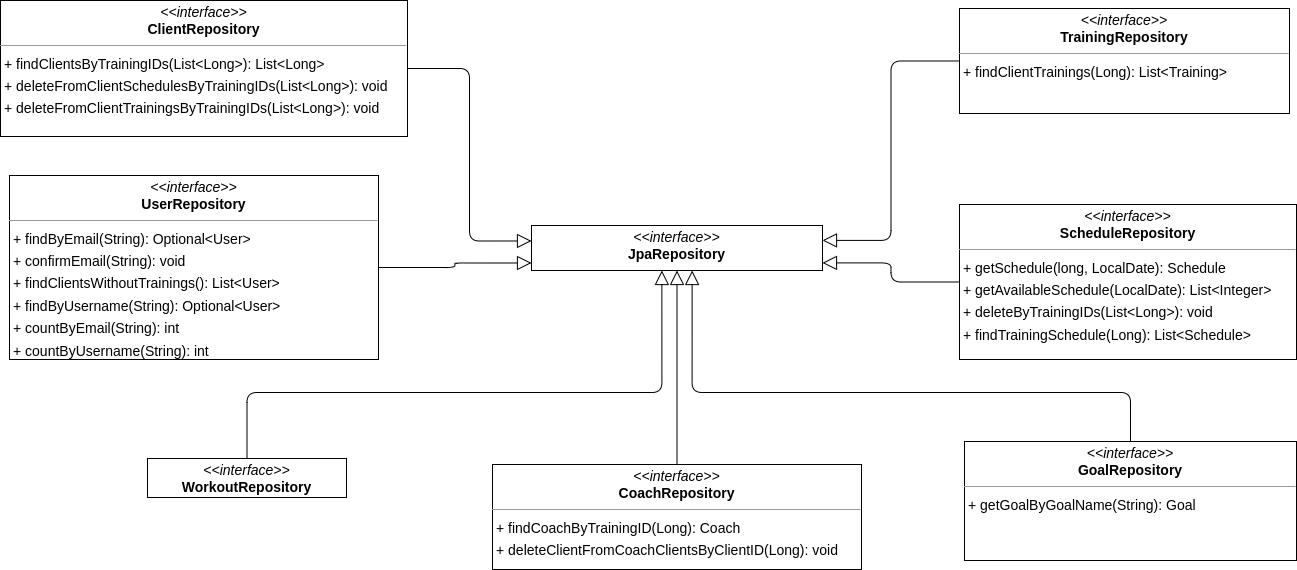
\includegraphics[scale=0.35]{./Dijagrami/repository.png}
		\centering
		\caption{Repozitoriji}
		\label{fig:promjene}
	\end{figure}
        \noindent Radi izbjegavanja zbijenosti na dijagramu servisa i repozitorija izdvojili smo razrede servisa i prikazali njihove implementirane funkcije na sljedećem dijagramu.
	\begin{figure}[H]
		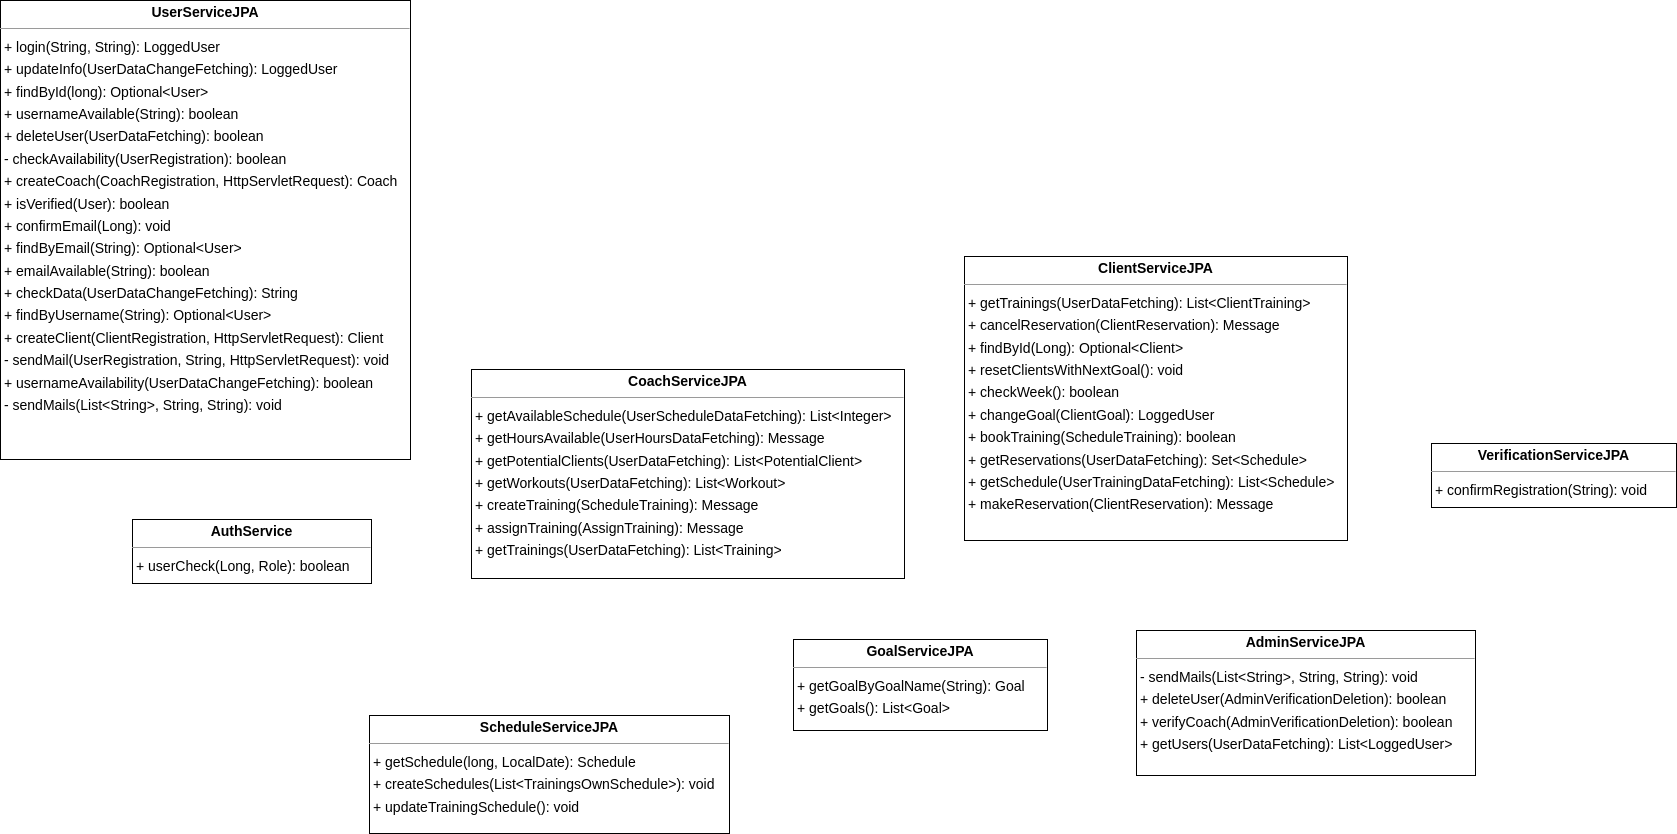
\includegraphics[scale=0.275]{./Dijagrami/services_methods.png}
		\centering
		\caption{Implementirane funkcije servisa}
		\label{fig:promjene}
	\end{figure}
	
		
		%\textbf{\textit{dio 2. revizije}}\\			
		
		%\textit{Prilikom druge predaje projekta dijagram razreda i opisi moraju odgovarati stvarnom stanju implementacije}
		
		
		
		%\eject
	
	%\section{Dijagram stanja}
		
		
	\noindent Dijagram stanja prikazuje stanja objekata te prijelaze među stanjima ovisno o događajima. Slika 4.9 prikazuje dijagram stanja za registriranog korisnika, točnije, vježbača. Prijavom u sustav otvara se početna stranica "Moj profil" na kojoj se mogu pregledati osobni podatci i obrisati račun. Početna stranica je, uz pregled treninga, pregled rezervacija i odjavu, vidljiva i dostupna iz svakog stanja. Na stranici pregleda treninga prikazani su svi treninzi dodijeljeni klijentu te postoji mogućnost odabira jednog od njih. Time se dobiva uvid u sve termine odabranog treninga koji se mogu rezervirati. Na stranici "Pregled rezervacija" prikazani su svi trenutno rezervirani termini logiranog vježbača koji se mogu i otkazati. Na stranici promjene korisničkih podataka dostupna je forma u koju se upisuju podatci za promjenu. 
  
	\begin{figure}[H]
		 \centering
		 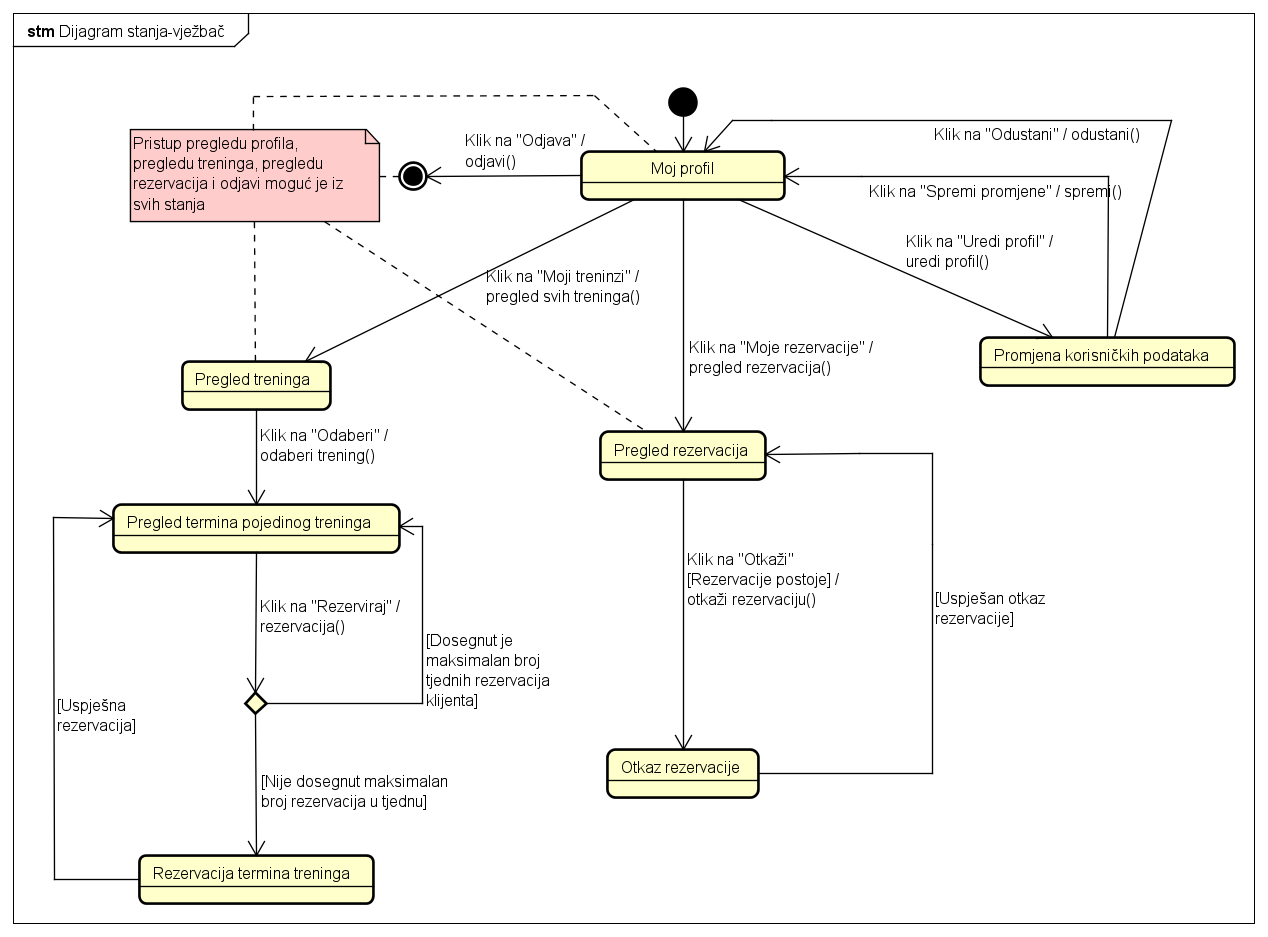
\includegraphics[width=\linewidth]{./Dijagrami/dijagramStanja-vjezbac.png}
		 \caption{Dijagram stanja}
		 \label{fig:Dijagram stanja}
	\end{figure}
		
		%\eject 
	
	%\section{Dijagram aktivnosti}
		
		%\textbf{\textit{dio 2. revizije}}\\
		
		 %\textit{Potrebno je priložiti dijagram aktivnosti s pripadajućim opisom. Dijagram aktivnosti treba prikazivati značajan dio sustava.}
        \noindent \newline Dijagram aktivnosti je ponašajni UML dijagram koji modelira ponašanje nizom akcija, a služi za detaljan prikaz upravljačkog i podatkovnog toga pojedinog segmenta aplikacije (najčešće pojedinih obrazaca uporabe). Dijagramom aktivnosti pogodno je opisivati sinkronizaciju i konkurentnost značajki. 
        \newline Uz našu aplikaciju implementirali smo dijagram aktivnost za obrazac uporabe 5:  „Promjeni korisničke podatke“ kako bismo prikazali podatkovni tok uređivanja postojećih korisničkih profila. 

        \begin{figure}[H]
		      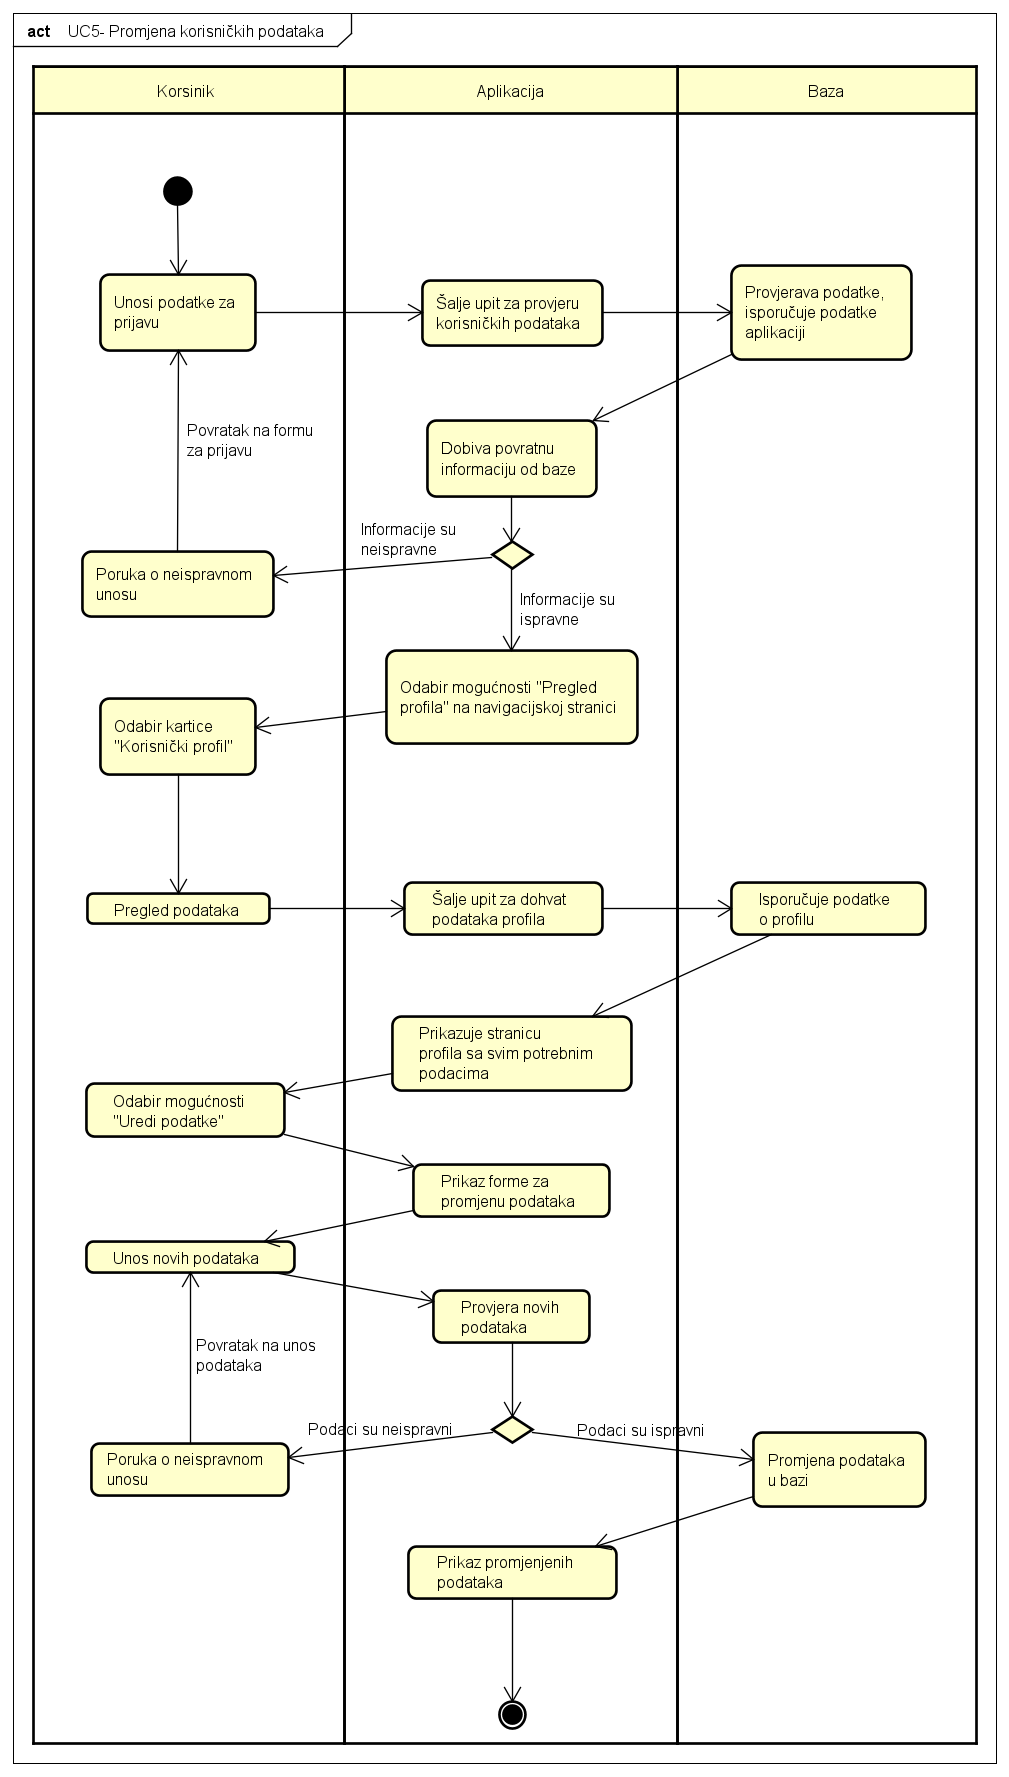
\includegraphics[scale=0.45]{./Dijagrami/UC5_Promjena_korisničkih_podataka_activity.png}
		      \centering
		      \caption{Dijagram aktivnosti za obrazac uporabe 5: "Promjena korisničkih podataka"}
		      \label{fig:promjene}
	   \end{figure}

		
		%\eject
	%\section{Dijagram komponenti}
	
		%\textbf{\textit{dio 2. revizije}}\\
	
		 %\textit{Potrebno je priložiti dijagram komponenti s pripadajućim opisom. Dijagram komponenti treba prikazivati strukturu cijele aplikacije.}

        \noindent \newline Dijagram komponenti je strukturni, statički UML dijagram koji vizualizira organizaciju i međuovisnost interne strukture implementacijskih komponenata, te odnos programske potpore prema okolini. Koristan je za stjecanje okvirne ideje o implementaciji sustava, bez ulaženja u prevelike detalje. 
        \newline Naša aplikacija podijeljena je u četiri glavne komponente: web preglednik (ciljana platforma za pogon aplikacije) koji dohvaća odgovarajuću frontend i backend logiku poštujući internetske komunikacijske protokole, frontend koji dohvaća odgovarajuće HTML, CSS i .js datoteke koje sadrže kod korisničkog sučelja, backend zadužen da dohvat i obradu podataka iz korisničkog sučelja i baze podataka i posreduje komunikaciji navedenih komponenti, te samu SQL bazu podataka.\newline Komponenti frontend logike pristupa se preko sučelja za dohvat HTML-a, CSS-s i .js datoteka iz web preglednika. Centralni dio frontenda je router datoteka (u našem slučaju App.js) zadužena za usklađivanje rada i dohvaćanje željenih komponenti koje su niže u hijerarhiji frontend logike. Svaka komponenta unutar frontend komponente na grafu sadržava ugnježđene komponente u čiju strukturu radi razumljivosti grafa ne ulazimo, a to označava da svaka komponenta ovisi o React libraryju. \newline Komponenta backend logike sa web preglednikom povezana je preko sučelja REST (zathjevi GET, POST, DELETE). Zahtjevi se nakon primitka prvo prosljeđuju kontrolerima, subkomponentama backenda zaduženim za prihvat i isporuku servisima. Servisi su subkomponente backenda koji pomoću svojih sučelja komuniciraju sa kontrolerima i prihvaćaju podatke koji se u njima nalaze, te ih pomoću JPA sučelja prosljeđuju repozitorijima. Repozitoriji omogućuju komunikaciju između servisa i baze podataka. Povezani su sučeljem s SQL bazom podataka. Prijenos podataka između komponenti backend logike ostvaren je „Data transfer object“ klasama pa sve komponente backenda imaju ovisnost prema njima. Svaka komponenta unutar backend komponente na grafu sadržava ugnježđene komponente u čiju strukturu radi razumljivosti grafa ne ulazimo, a to označava da svaka komponenta ovisi o Spring libraryju. 

        \begin{figure}[H]
		    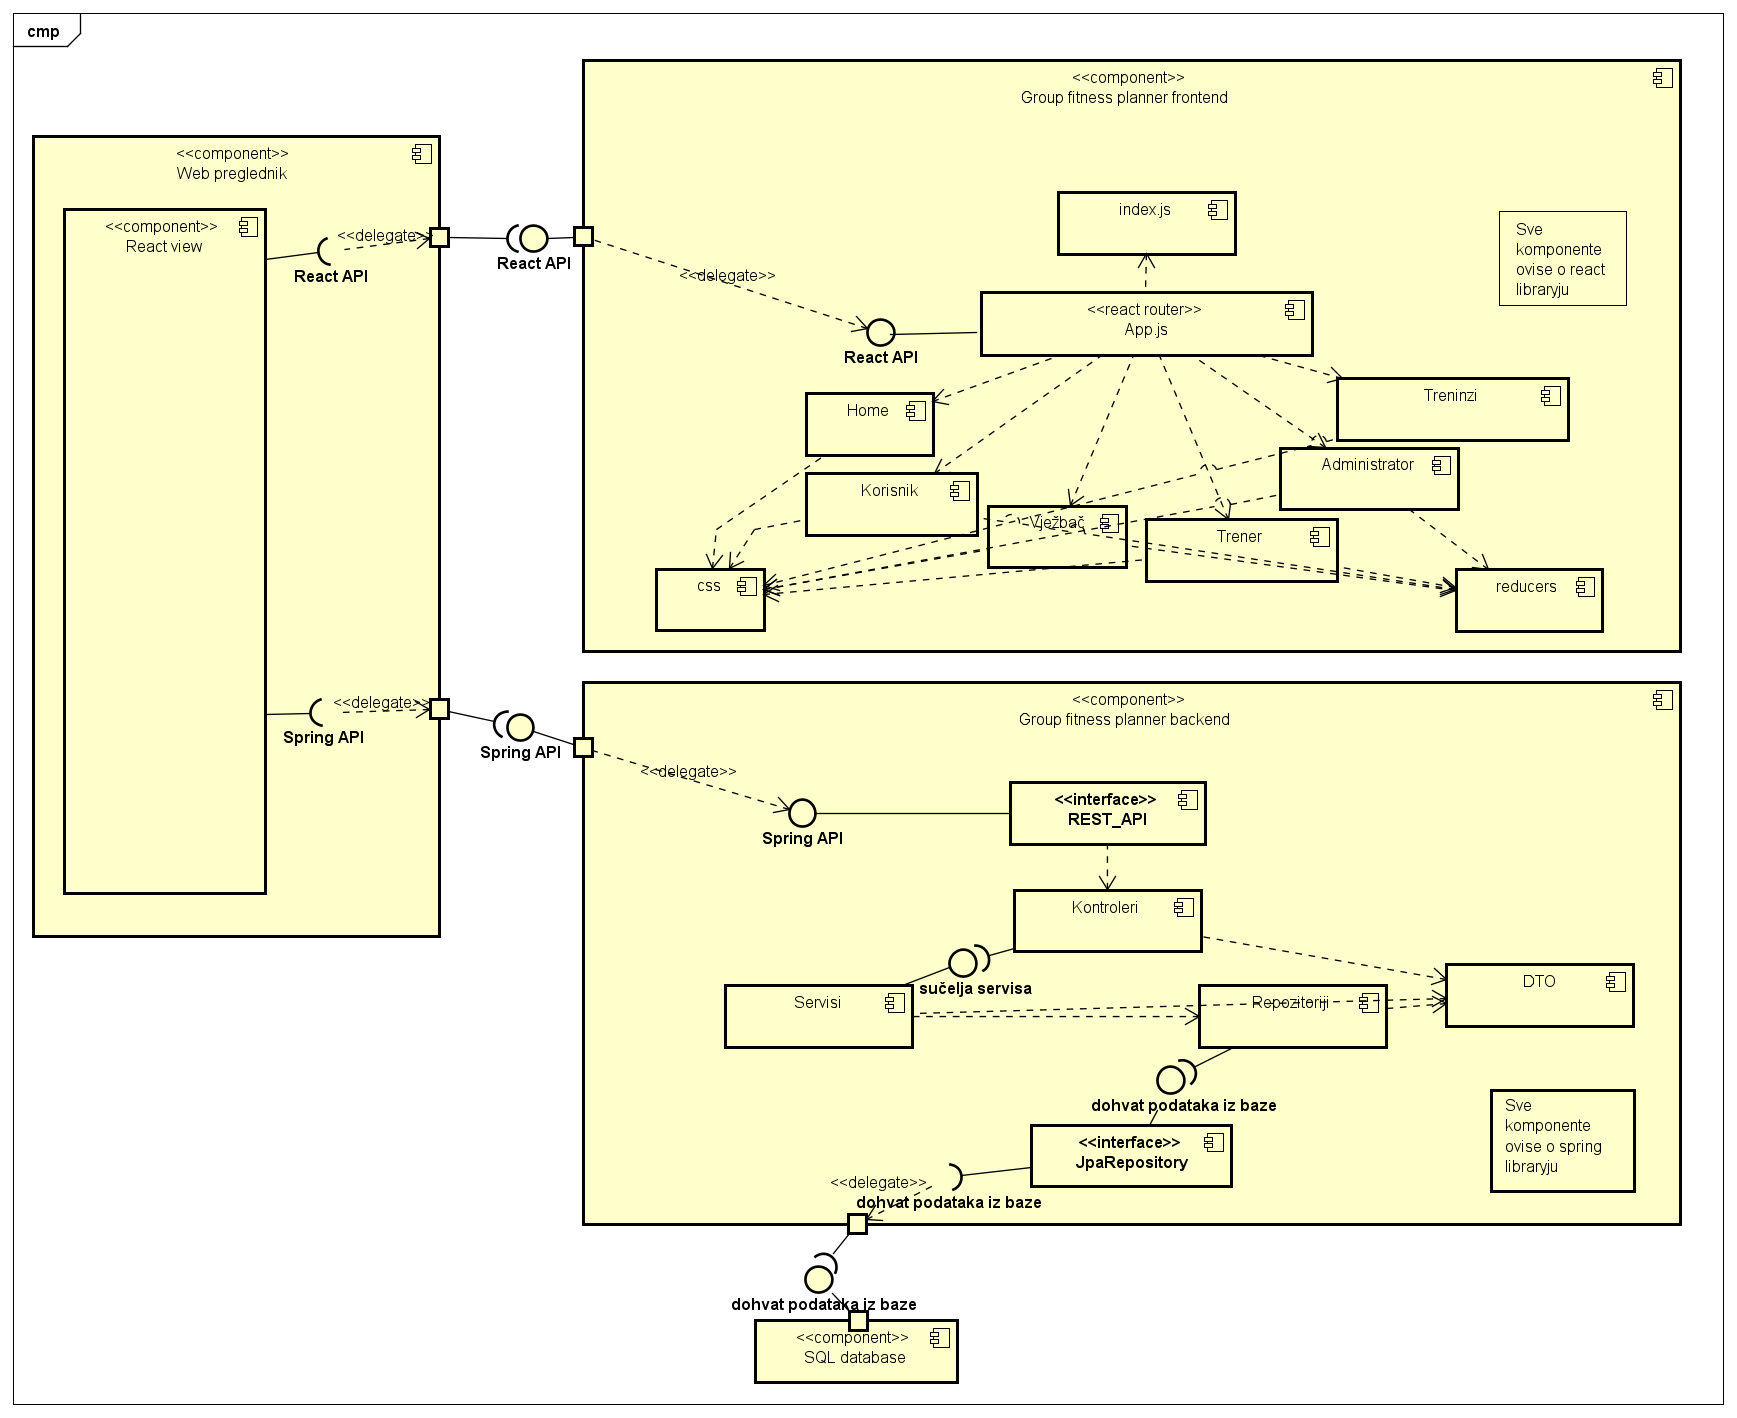
\includegraphics [scale=0.35]{./Dijagrami/Dijagram_komponenti.png}
		      \centering
		      \caption{Dijagram komponenti aplikacije}
		      \label{fig:promjene}
	   \end{figure}
